\part{Ayudantia 2}

\section{Parte 1}

Si tenemos un caso donde conocemos 2 puntos a alturas distinta:

\begin{figure}[H]
    \centering
    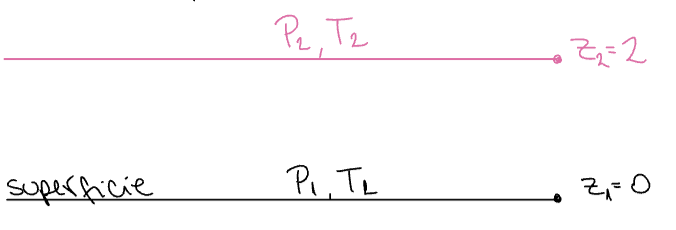
\includegraphics[width=0.5\textwidth]{imagenes/ayud_2_1.png}
    \label{fig:altura}
\end{figure}

Podemos determinar el agua precipitable se utiliza la siguiente formula:

\begin{equation}
    \Delta m_p = q_v \cdot p_a \cdot A \cdot \Delta Z
\end{equation}

$q_v$ se define como:

\begin{equation}
    q_v = 0.622 \cdot \frac{e}{p_a}
\end{equation}

Donde e es la presion de vapor y $p_a$ es la presion atmosferica.
\\ \\ 
Ademas, se tiene lo siguiente:

\begin{equation}
    HR = \frac{e}{e_s} \cdot 100
\end{equation}

Donde HR es la humedad relativa y $e_s$ es la presion de vapor de saturacion, de lo cual se obtiene:

\begin{equation}
    e_s = 611^(\frac{17.27 \cdot T}{237.3 + T})
\end{equation}

Los valores de e y $e_s$ son en pascales, donde las temperaturas son ingresadas en celcius.
\\ \\
Donde podemos calcular la presion del punto mas alto en variacion al punto base de referencia:

\begin{equation}
    P2 = P1 \cdot (\frac{T2}{T1})^(\frac{g}{\alpha \cdot Ra})
\end{equation}

Donde $\alpha$ ($\frac{C}{Km}$) es el gradiente de temperatura, Ra $\frac{J}{Kg \cdot K}$ es la constante de los gases y g es la gravedad.
\\ \\
Podemos conocer la temparatura en el punto de segun la temparatura en el punto 1:

\begin{equation}
    T2 = T1 + \alpha \cdot \Delta Z
\end{equation}

Ademas, es nesesario calcular la presion en el punto base de referencia segun la Ra y T:

\begin{equation}
    P1 = \frac{P1}{Ra \cdot T1}
\end{equation}

Lo mismo es nesesario hacer con P2.
\\ \\
Luego, como en este caso hay 2 puntos, hay que sacar el promedio de $q_v$ y Pa, obteniendo asi $\Delta m_p$.  

\section{Parte 2}

Podemos obtener la vida util a partil de la seguridad:

\begin{equation}
    S = (1 - \frac{1}{T})^n
\end{equation}

\subsection{Gumbell}

Se define Gumbell como:

\begin{equation}
    X_T = \mu + K_t \cdot \sigma
\end{equation}

\begin{equation}
    K_t = \frac{y_t - y_n}{\sigma_n}
\end{equation}

\begin{equation}
    y_t = -\ln(\ln(\frac{T}{T-1}))
\end{equation}

Los valores n deben ser entregados.
\\ \\
La probabilidad de que la estructura falle mas de \textbf{X} veces es:

\begin{equation}
    P(X_{fallas}) = 1 - P(0) + P(1) + P(2) + ... + P(X-1)
\end{equation}

Aplicando la distribucion de bernoulli:

\begin{equation}
    P(k) = \binom{n}{k} \cdot P^k \cdot (1-P)^{n-k}
\end{equation}

Donde \textbf{k es el numero de fallas} y \textbf{P las probabilidades de excedencia}.

\begin{equation}
    \binom{n}{k} = \frac{n!}{k!(n-k)!}
\end{equation}

\subsection{Log Pearson III}

Se define como:

\begin{equation}
    X_T = \mu + K_t \cdot \sigma
\end{equation}

\begin{equation}
    K_t = Z + (Z^2 - 1)K + \frac{1}{3}(Z^3 - 6Z)K^2 - (Z^2-1)Z^3 + Z\cdot K^4 + \frac{K^5}{3}
\end{equation}

\begin{equation}
    K = \frac{CS}{6}
\end{equation}

Donde CS es el coeficiente de simetria.
\\ \\
Z se calcula de acuerdo a la distribucion normal:

\begin{equation}
    Z = W -  \frac{2.516 + 0.803W + 0.0103W^2}{1 + 1.432W + 0.189W^2 + 0.001308W^3}
\end{equation}

\begin{equation}
    W = (\ln(\frac{1}{P^2}))^{0.5}
\end{equation}

\begin{equation}
    P = \frac{1}{T}
\end{equation}

\subsection{Caudal de Diseño}

Luego usando las distintas distribuciones, se define el caudal de diseño como:

\begin{equation}
    Q_{diseno} = \exp(X_T)
\end{equation}

\subsection{Intervalos de Confianza}

Se define como:

\begin{equation}
    X_t + - S_e \cdot Z_{\alpha}
\end{equation}

\textbf{$Z_{\alpha}$} es la variable normal estandar para un nivel de confianza de $\alpha$. Para $\alpha$ = 5 \%, implica que $Z_{\alpha}$ = 1.96. = 1.645. Luego:

\begin{equation}
    S_e = \sqrt{(1+1.139K_t + 1.1000K_t^2) \cdot \frac{1}{n}}
\end{equation}

De esta forma, obtenemos los 2 limites del intervalo de confianza.